\chapter{Comparison of Knowledge Tracing Methods}

\section{Data Description}\label{sec:kt_data}
We use four publicly available datasets, three of which are standard in the knowledge tracing literature. Two of the four datasets are simulated according to IRT models to demonstrate the capability of our IRT-inspired knowledge tracing methods to learn the IRT model parameters. We also include two real-world datasets common in knowledge tracing literature. A summary of each dataset is given in Table \ref{tab:kt_data}.

\subsubsection*{Synth-5}\footnote{https://github.com/chrispiech/DeepKnowledgeTracing/tree/master/data/synthetic}
This dataset was generated by Piech et al. \cite{piech2015} for experiments with DKT. There are 50 items covering 5 latent concepts. Each item requires exactly one concept, and responses are generated according to the Rasch model \cite{lord1968} with guessing: 
\begin{equation}
  P(u_{ij} = 1| \Theta_j; b_i) = c + \frac{1-c}{1 + e^{b_i - \theta_{jk}}}
  \label{eq:rasch_guess}
\end{equation}
The guessing parameter $c$ is fixed at $0.25$. Note that in Equation \ref{eq:rasch_guess}, only a single skill $k$ is referenced when answering item $i$. Responses to each of the 50 items are simulated for 4,000 students.

\subsubsection*{Sim200}\footnote{https://github.com/converseg/irt\_data\_repo/tree/master/sim200}
Sim200 differs from Synth-5 in a few important ways. First, there are more items (200) and more latent skills (20). Second, the $Q$-matrix is more dense -- items require multiple skills in order for students to answer correctly. Each entry in the $Q$-matrix was sampled from $\text{Bern}(0.2)$. Lastly, Sim200 generates responses according to the ML2P model in Equation \ref{eq:ml2p}, as opposed to the Rasch model. The item parameters were taken from a random uniform distribution; the difficulty parameters from $b_i \in [-3,3]$ and the nonzero discrimination parameters from $a_{ik} \in [0.1,0.9]$. This dataset is similar to the Sim-20 dataset described in Section \ref{sec:irt_data}, but the latent abilities $\Theta$ were generated according to a standard normal Gaussian distribution.

\subsubsection*{Statics2011}\footnote{https://pslcdatashop.web.cmu.edu/DatasetInfo?datasetId=507}
Statics is a real-world dataset with responses from 316 students enrolled in a college engineering course. After formatting the data, the dataset includes 987 unique items and 61 latent concepts. Students answered varying amounts of questions, with a total of 135,338 distinct interactions.

\subsubsection*{Assist2017}\footnote{https://sites.google.com/view/assistmentsdatamining}
The ASSISTments 2017 dataset contains real-world interactions from 1,709 students recorded on the ASSISTments online tutoring system. There is a large number of distinct items (4,117), and 102 latent concepts. Some items are tagged with the concept ``noskill'' -- we treat this tag as a latent concept, otherwise all interactions involving such items would need to be thrown out.

\begin{table}
  \centering
  \begin{tabular}{l c c c c}
    \hline
    Dataset & Items & Skills & Students & Interactions \\
    \hline
    Synth-5 & 50 & 5 & 4,000 & 20K \\
    Sim200 & 200 & 20 & 50,000 & 10M \\
    Statics2011 & 987 & 61 & 316 & 135K \\
    Assist2017 & 4,117 & 102 & 1,709 & 392K \\
  \end{tabular}
  \caption{Summary of datasets.}
  \label{tab:kt_data}
\end{table}


\section{Experiment Details}
In the two simulated datasets (Synth-5 and Sim200), all students answering the same set of questions and thus all have the same length of response sequences (50 and 200, respectively). On Statics2011 and Assist2017, the maximum sequence length is set at $L=128$, and student's whose response sequences are longer/shorter than 128 interactions have their response sequences wrapped/padded. The rest of the hyper-parameters are described in Table \ref{tab:kt_params}. The hyperparameters for DKT, SAKT, and DKVMN follow those reported in the corresponding literature.

\begin{table}
  \centering
  \begin{tabular}{l c c c c c}
    \hline
    Parameter & Synth-5 & Sim200 & Statics2011 & Assist2017 \\
    \hline
    max\_len & 50 & 200 & 128 & 128 \\
    input\_size & 101 & 201 & 1975 & 8235 \\
    output\_size & 50 & 200 & 987 & 4117 \\
    hid\_size & 64 & 64 & 50 & 100 \\
    skill\_layer & 5 & 20 & 61 & 102 
  \end{tabular}
  \caption{Hyper-parameters used in DKT-IRT and SAKT-IRT on each dataset.}
  \label{tab:kt_params}
\end{table}

\section{Results}

As seen in Table \ref{tab:kt_results}, the two IRT-inspired knowledge tracing methods methods (DKT-IRT and SAKT-IRT) are able to produce AUC values competitive with other deep learning methods. As expected, the sacrifice in accuracy is smaller in simulated datasets. In Synth-5 and Sim200, the responses were generated with known IRT models which match the architecture of IRT-inspired methods. 

\begin{table}
  \centering
  \begin{tabular}{l c c c c}
    \hline
    Method & Synth-5 & Sim200 & Statics2011 & Assist2017 \\
    \hline 
    DKT & 0.803 & 0.838 & 0.793 & 0.731 \\
    SAKT & 0.801 & 0.834 & 0.791  & 0.754 \\
    DKVMN & 0.827 & 0.829 & 0.805 & 0.796 \\
    \textbf{DKT-IRT} & 0.799 & 0.824 & 0.777 & 0.724 \\
    \textbf{SAKT-IRT} & 0.798 & 0.833 & 0.775 & 0.728
  \end{tabular}
  \caption{TestAUC values for various models on each dataset.}
  \label{tab:kt_results}
\end{table}

Note that when working on Synth-5, we know that there were no discrimination parameters used to generate the data. As such, we fix all nonzero weights in the output layer to be equal to one by replacing Equation \ref{eq:weight_constraint} with $W_p = Q$. We do not incorporate any estimation or knowledge of the guessing parameter $c$ into the knowledge tracing model. This may account for a larger discrepancy in AUC between our methods and DKVMN in Synth-5 than seen in the Sim200 data.

When looking at the two real-world datasets, the trade-off in AUC is more significant, as it is not known if the student responses follow the ML2P model. There could also be inaccuracies in the given item-skill association $Q$-matrix, which our models are dependent on. Additional difficulties arise in the Assist2017 data, discussed in Section \ref{sec:kt_data}, concerning exercise-skill tags may explain the considerable performance gap between IRT-inspired methods and DKVMN on this dataset.

\begin{figure}[h]
  \centering
  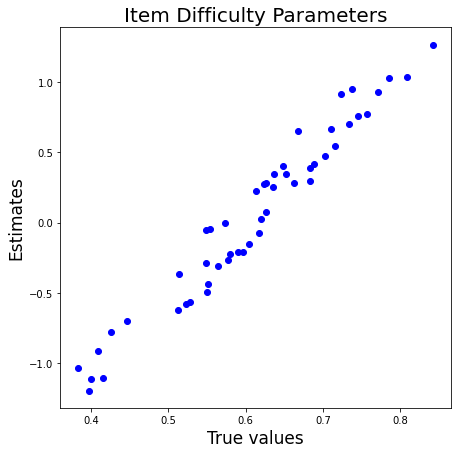
\includegraphics[width=.5\textwidth]{img/kt_irt/synth5_diff_est_lstm.png}
  \caption{Correlation between DKT-IRT estimates and true values of Synth-5 item difficulty. SAKT-IRT produced similar results.}
  \label{fig:synth5_diff}
\end{figure}

A comparison between the output layer bias parameters and true item difficulty parameters is shown in Figure \ref{fig:synth5_diff}. This displays high correlation, and the trainable bias parameters in the output layer can be interpreted as approximations of the item difficulty parameters. Due to the available public dataset, there is no access to the true values of student abilities $\Theta$.

\begin{figure}[h]
  \centering
  \minipage{.5\textwidth}
  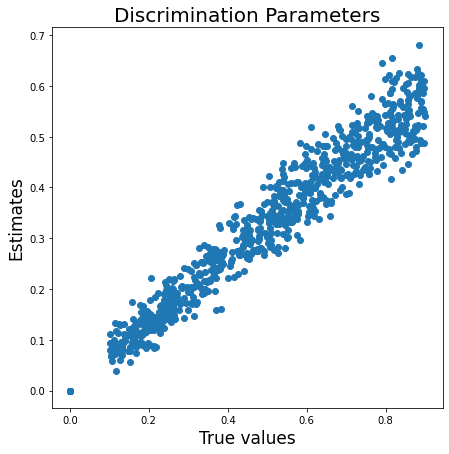
\includegraphics[width=.85\textwidth]{img/kt_irt/disc_est_attn2.png}
  \endminipage
  \minipage{.5\textwidth}
  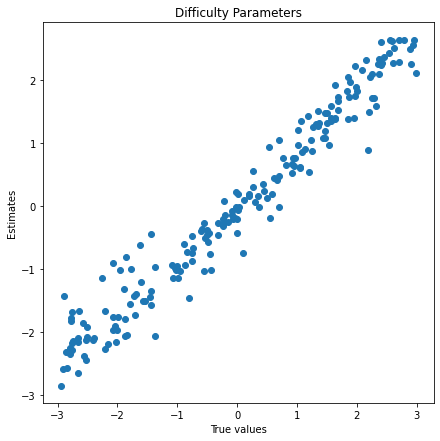
\includegraphics[width=.85\textwidth]{img/kt_irt/diff_attn_sim200.png}
  \endminipage
  \caption{Correlation between true and estimated Sim200 (left) item discrimination parameters, and (right) item difficulty parameters.}
  \label{fig:disc_diff_sim200}
\end{figure}

The parameter estimates can be directly compared to the true parameters in the Sim200 dataset. In Figure \ref{fig:disc_diff_sim200}, we can see the true values of item discrimination parameters $a_{ik}$ and item difficulty parameter. The correlation here is very high, and the estimates for item parameters are quite accurate. The student ability parameters $\theta_{jk}$ plotted against estimates given by SAKT-IRT at the final timestep in Figure \ref{fig:theta_sim200}. While there is a lot more noise in the student ability estimates, there is still significant correlation with the true values. 

It is important to note that the estimates to $\Theta$ do not require any additional computations or transformations and are directly obtained from the nerual network. This is an advantage over other deep knowledge tracing methods, which only output the probability of answering items correctly and require other methods of quantifying knowledge concepts. Recall that while estimates to student ability are the neuron activation values at the skill layer from feeding forward a response sequence, the discrimination parameter estimates are the trained weights connecting the skill layer to the output layer.

\begin{figure}[h]
  \centering
  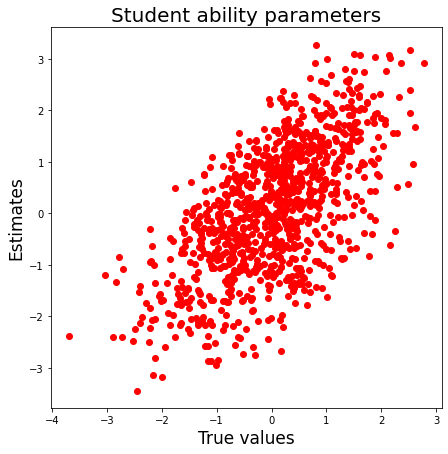
\includegraphics[width=.5\textwidth]{img/kt_irt/theta_est_attn2.png}
  \caption{Correlation between true and estimated student ability parameters at $t=L=200$ for the Sim200 dataset.}
  \label{fig:theta_sim200}
\end{figure}

\begin{figure}[h]
  \centering
  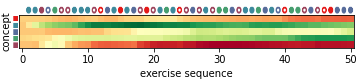
\includegraphics[width=.7\textwidth]{img/kt_irt/knowledge_trace_lstm_edited.png}\\
  \vspace{.5cm}
  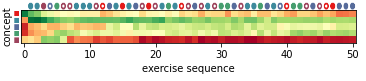
\includegraphics[width=.7\textwidth]{img/kt_irt/knowledge_trace_attn_edited.png}
  \caption{Tracing a student's knowledge mastery with DKT-IRT (top) and SAKT-IRT (bottom) as they progress through the items of the Synthetic-5 dataset.}
  \label{fig:synth5_trace}
\end{figure}

The explcit representation of knowledge $\Theta$ makes tracing student progress over time very convenient. For student $j$'s response sequence of length $L$, IRT-inspired knowledge tracing methods return a $K \times (L+1)$ matrix, where the entry $(k,t)$ gives the latent trait estimate to the $k$-th skill at time $t$, $\theta_{jkt}$. This is visualized in Figure \ref{fig:synth5_trace} on the Synth-5 dataset. Notice how a correct response in a skill (filled-in circle) corresponds with a more green and less red skill value. Likewise, an incorrect response in a skill (hollow circle) corresponds with a more red skill or less green skill value. When comparing the knowledge tracing from DKT-IRT and SAKT-IRT, the DKT-IRT tracing is much more smooth as a student moves through the exam. This is likely because of the recurrent structure of an LSTM: the skill values at time $t$ are only directly related to the values at time $t-1$. The SAKT-IRT tracing graphic is much choppier, because the attention mechanism does not have recurrent structure and instead maintains connections to all previous interactions.


\section{Discussion}
The connection between IRT and knowledge tracing presented in this work introduces a trade-off between accuracy and interpretability. Further work to increase AUC to the level of DKVMN while maintaining explainability is worth exploring. Though IRT-inspired knowledge tracing does require an expert to annotate the item-skill association $Q$-matrix while other methods do not, explicitly incorporating this information greatly increases the ability to interpret a deep learning model. Further, most intelligent tutoring systems provide an item-skill tag, so availability of the $Q$-matrix is not an unreasonable assumption.

Our proposed method's ability to function as both a knowledge tracing model while also estimating item parameters gives it a unique interpretation rooted in Item Response Theory. This link with IRT is helpful in practice, because it provides an explicit and easy to obtain quantity for a student's latent abilities. This approximation of a student ability can be interpreted in the frame of IRT, as opposed to only a prediction of correctness for each item. This is a clear advantage that IRT-inspired knowledge tracing has over conventional non-interpretable deep learning methods.

